\documentclass{article}

\usepackage[nonatbib, final]{neurips}
\usepackage[numbers]{natbib}

\makeatletter
\renewcommand{\@noticestring}{
  \centering
  
}
\makeatother

% Minimal packages for the paper — no algorithm2e, no tabularray
\usepackage[T1]{fontenc}
\usepackage{hyperref}
\usepackage{microtype}
\usepackage{xcolor}
\usepackage{graphicx}
\usepackage{booktabs}
\usepackage{amsmath, amsfonts}
% nicefrac not available in basic TeX — use \nicefrac replacement if needed

% Custom footnote symbols
\makeatletter
\newcommand{\ssymbol}[1]{\@fnsymbol{#1}}
\newcommand{\romanNumeral}[1]{\expandafter\@slowromancap\romannumeral #1@}
\makeatother


% physics.sty not available — using amsmath directly
\usepackage{mathtools}
\usepackage{booktabs}
\usepackage{microtype}
\usepackage{xcolor}
\usepackage{hyperref}

\DeclarePairedDelimiter\p{(}{)}
\DeclarePairedDelimiter\n{|}{|}
\DeclarePairedDelimiter\B{[}{]}

\title{Predicting the Energy of a Complete LLM Data-Curation Pipeline on Shared HPC}

\author{
  Romir Malik\thanks{Utrecht University.} \quad
  Julio de Oliveira Filho\thanks{TNO.} \quad
  Martino Mensio\footnotemark[2] \quad
  Lisa Bylinina\footnotemark[1]
}

\begin{document}

\maketitle

\begin{abstract}
Before committing a multi-day data-curation job for an LLM corpus, a team needs one number: how much energy will the \emph{whole} pipeline consume? We run the complete four-stage GPT-NL curation pipeline --- document splitting, string normalisation, heuristic filtering, and deduplication --- on the Snellius supercomputer and build a predictor for its total energy from cheap trial runs. Two obstacles make this hard, and both are measured rather than assumed: the Energy Aware Runtime (EAR) telemetry that reports per-job power is contaminated by co-tenants on shared nodes (node-level readings inflate by up to $2.4\times$), and the deduplication stage initially emitted no energy record at all.
We calibrate a two-parameter linear energy model per stage from small exclusive runs (minutes), then walk the pipeline with an Extended Kalman Filter whose innovation gate tests each incoming reading: clean readings tighten the prediction intervals (Mode~B), while contaminated or missing readings are rejected and replaced by the model with widened uncertainty (Mode~C). Across all four stages, held-out prediction $R^2$ ranges $0.73$--$0.96$ (vs.\ in-sample ${\ge}0.997$), and the gate cuts a contaminated shared-node reading's $+93\%$ pipeline error to $+8\%$. Deduplication, once its telemetry was fixed, was swept on exclusive nodes at $1$k--$400$k documents (clean $34.8$\,kJ at $100$k; the contaminated single run had over-read it by $1.8\times$); the $1.4$M run runs out of memory in the MinHash signature pass --- the one stage in the pipeline that does not scale. Energy per \emph{character} is nearly invariant (${\approx}4{\times}10^{-4}$\,J/char across a $256\times$ document-length range), making the prior portable across corpora; and replacing contaminated power with a time-derived estimate ($E = P^{\mathrm{eff}}\cdot t$, wall-time being co-tenancy-invariant) drops shared-node error from $45.8\%$ to $5.4\%$. The result is a full-pipeline energy account that stays accurate when the measurement layer is partially broken.
\end{abstract}

% ===========================================================================
\section{Introduction}
% ===========================================================================

The energy reporting for large language models concentrates on training and inference \cite{strubell2019energy,patterson2021carbon}. The step that comes before both --- \emph{data curation}, the multi-stage pipeline that splits, normalises, filters, and deduplicates raw text into a training corpus --- is run over hundreds of millions of documents, yet its energy cost is almost never reported, and to our knowledge never predicted before a run.

We work inside the GPT-NL project, a Dutch--English foundation-model effort whose curation pipeline runs on the Snellius national supercomputer \cite{surf_snellius}. The pipeline has four CPU stages --- \texttt{data\_splitting}, \texttt{string\_normalization}, \texttt{heuristic\_filtering}, and \texttt{deduplication} --- and is instrumented with the Energy Aware Runtime (EAR), a hardware-level monitoring stack from the Barcelona Supercomputing Center \cite{bsc_ear} that records per-job DC node power, CPU utilisation, and memory bandwidth at sub-second granularity. The practical need is concrete: before launching a multi-day curation job over a new corpus, the team wants a \emph{whole-pipeline} energy estimate --- the sum over all four stages --- with an honest error bar, obtained \emph{cheaply} from small trial runs that finish in minutes. This means we cannot quietly drop the stage that is awkward to measure; the total has to include it.

The obstacle is that on a shared HPC cluster, EAR telemetry is \textbf{unreliable} in two distinct ways that surfaced as we ran the full pipeline:

\begin{enumerate}
  \item \textbf{Contaminated.} Node-level DC power includes co-tenant workloads. We ran a controlled experiment: the same stage, same corpus, same size, run once with the node to itself (exclusive) and once with neighbours on the remaining cores (shared). Wall time and CPU utilisation were identical (595\,s, 97\%); measured power was $2.4\times$ higher on the shared run (669\,W vs.\ 275\,W) --- the difference is the neighbours, not the job (\S\ref{sec:controlled}).
  \item \textbf{Missing.} The deduplication stage runs as four chained sub-jobs (signature, buckets, cluster, filter) that, in the EAR configuration we inherited, never emitted an energy record --- the sub-job launcher did not create the directory EAR writes to. A one-line fix recovers them, after which we swept the stage on exclusive nodes (\S\ref{sec:results-dedup}).
\end{enumerate}

A naive estimator that trusts every EAR reading inherits both failures: a $+93\%$ over-estimate when it swallows a contaminated reading, and an incomplete total when a stage reports nothing. We want a calibrated whole-pipeline total with honest uncertainty \emph{despite} the measurement layer being partially absent or corrupted.

\textbf{Our approach.} For each of the four stages we (i)~calibrate a two-parameter linear energy model from cheap exclusive-node runs, then (ii)~walk the pipeline sequentially with an Extended Kalman Filter (EKF) whose innovation gate decides, at each stage, whether to trust the incoming EAR reading or fall back to the model. The pipeline total is the sum of the stage estimates.

\textbf{Contributions.}
\begin{enumerate}
  \item \textbf{A full-pipeline energy account.} We calibrate and validate per-stage energy models for \emph{all four} stages of the GPT-NL pipeline across corpus sizes spanning $10^3$ to $1.4{\times}10^6$ documents. Held-out prediction $R^2$ ranges $0.73$--$0.96$; in-sample $R^2 \ge 0.997$ is shown to be systematically misleading (\S\ref{sec:results-heldout}). Running the whole pipeline also exposes the one stage that does not scale: deduplication's MinHash signature pass runs out of memory at $1.4$M documents (\S\ref{sec:results-dedup}).
  \item \textbf{A telemetry-robust sequential estimator.} The EKF runs each stage in one of three modes --- predict (no telemetry yet), update (clean reading absorbed, intervals tighten), reject/impute (contaminated or missing reading replaced by the model, uncertainty widened) --- chosen \emph{automatically} by an innovation gate that tests statistical consistency with the calibrated prior. The gate cuts a contaminated reading's $+93\%$ pipeline error to $+8\%$ (\S\ref{sec:ekf}, \S\ref{sec:results-ekf}).
  \item \textbf{Shared-node resolution via wall-time.} Wall clock time is co-tenancy-invariant, and $E = P^{\mathrm{eff}} \cdot t$ with a once-calibrated effective power reduces shared-node prediction error from $45.8\%$ to $5.4\%$ (\S\ref{sec:results-shared}).
  \item \textbf{Cross-corpus transfer via character invariance.} A second corpus with $256\times$ longer documents reveals that energy per \emph{character} is nearly corpus-invariant (${\approx}4{\times}10^{-4}$\,J/char for the dominant stage), making the prior portable across corpora without re-measurement (\S\ref{sec:results-chars}).
\end{enumerate}

% ===========================================================================
\section{Method}
% ===========================================================================

\subsection{Per-stage calibration}

\label{sec:calibration}

Let stage $s$ process $n$ input documents. We model its energy as
\begin{equation}
  E_s(n) = c_0^{(s)} + c_1^{(s)} \cdot n + \varepsilon_s,
  \qquad \varepsilon_s \sim \mathcal{N}(0, \sigma_s^2),
  \label{eq:linear}
\end{equation}
where $c_0$ is the fixed start-up cost (process launch, framework initialisation) and $c_1$ is the marginal energy per document. We fit Eq.~\eqref{eq:linear} from a small set of exclusive-node calibration runs spanning two orders of magnitude in $n$. With $m$ calibration measurements per stage ($m = 8$ in our experiments: 4 sizes $\times$ 2 replicates), the design matrix $X \in \mathbb{R}^{m \times 2}$ has rows $[n_i, 1]$ and target vector $y \in \mathbb{R}^m$ holds measured energies. We solve
\begin{equation}
  \hat{\theta}_s = (X^\top X + \lambda I')^{-1} X^\top y,
  \qquad \theta_s = (c_1, c_0)^\top,
  \label{eq:ridge}
\end{equation}
with a small ridge penalty ($\lambda$, chosen by leave-one-replicate-out cross-validation) on the slope only ($I' = \mathrm{diag}(1,0)$). The residual variance is $\hat{\sigma}_s^2 = \|y - X\hat{\theta}_s\|^2 / (m-2)$, yielding a closed-form coefficient covariance $\mathrm{Cov}(\hat{\theta}_s) = \hat{\sigma}_s^2 (X^\top X + \lambda I')^{-1}$. For a new corpus size $n_\star$, the prediction interval is
\begin{equation}
  \hat{E}_s(n_\star) \pm t_{0.975, m-2} \cdot \hat{\sigma}_s \sqrt{1 + x_\star^\top (X^\top X + \lambda I')^{-1} x_\star},
  \label{eq:predint}
\end{equation}
where $x_\star = [n_\star, 1]$. The $1+$ inside the square root separates fitting uncertainty (leverage) from irreducible measurement noise. This analytical interval is exact and propagates cleanly into the pipeline estimator --- the reason we keep the model linear.

\textbf{The metric that matters.} The $R^2$ of Eq.~\eqref{eq:ridge} on \emph{all} calibration sizes measures how well the line describes data it has already seen. That is not what we care about. We care whether a model calibrated on \emph{cheap, small} runs predicts an \emph{expensive, large} one. We therefore split the sizes:
\[
  \underbrace{\{10^3, 10^5\}}_{\text{calibrate}}
  \longrightarrow
  \underbrace{\{4{\times}10^5, 1.4{\times}10^6\}}_{\text{predict}},
\]
fit on the calibration sizes only, and report held-out prediction $R^2$ and mean relative error (MRE). This directly operationalises the ``predict the full run from a quick sample'' claim.

\subsection{The Kalman walk}

\label{sec:ekf}

The pipeline is a chain: stage $s$ outputs $n_{s+1} = r_s \cdot n_s$ documents, where the survival rate $r_s$ is observed from output Parquet files after stage $s$ completes. We track a two-dimensional state vector after stage $s$:
\begin{equation}
  \mathbf{x}_s = \begin{bmatrix} n_s \\ E_{\mathrm{cum},s} \end{bmatrix},
  \qquad
  P_s = \begin{bmatrix} \sigma^2_{n,s} & \sigma_{nE,s} \\ \sigma_{nE,s} & \sigma^2_{E,s} \end{bmatrix},
  \label{eq:state}
\end{equation}
where $n_s$ is the surviving document count and $E_{\mathrm{cum},s}$ is the cumulative energy consumed through stage $s$. The initial state is $\mathbf{x}_0 = [n_0, 0]^\top$ with $P_0 = \mathrm{diag}(\sigma^2_{n_0}, 0)$.

\textbf{Predict step (before stage $s+1$).} We propagate the state forward using the calibrated model and the survival rate:
\begin{equation}
  \hat{\mathbf{x}}_{s+1|s} = f_s(\hat{\mathbf{x}}_{s|s}) =
  \begin{bmatrix}
    r_s \cdot n_s \\
    E_{\mathrm{cum},s} + c_0^{(s+1)} + c_1^{(s+1)} \cdot n_{s+1}
  \end{bmatrix}.
  \label{eq:transition}
\end{equation}
The covariance is propagated through the Jacobian $F_s = \partial f_s / \partial \mathbf{x}$:
\begin{equation}
  P_{s+1|s} = F_s P_{s|s} F_s^\top + Q_{s+1},
  \qquad
  F_s = \begin{bmatrix} r_s & 0 \\ c_1^{(s+1)} r_s & 1 \end{bmatrix},
  \label{eq:covprop}
\end{equation}
where the process noise $Q_{s+1}$ encodes the OLS prediction variance from Eq.~\eqref{eq:predint} and survival-rate uncertainty.

\textbf{Update step (after stage $s+1$ completes).} EAR reports an energy $z_{s+1}$. The innovation (observation minus prediction) is
\begin{equation}
  y_{s+1} = z_{s+1} - H \hat{\mathbf{x}}_{s+1|s},
  \qquad H = [0, 1].
  \label{eq:innovation}
\end{equation}

\textbf{Mode selection --- the innovation gate.} A reading is accepted (Mode~B) iff it is statistically consistent with the calibrated model:
\begin{equation}
  y_{s+1}^2 \le \gamma^2 \cdot S_{s+1},
  \qquad S_{s+1} = H P_{s+1|s} H^\top + \sigma^2_{\mathrm{EAR}},
  \label{eq:gate}
\end{equation}
where $\gamma = 3$ (a $3\sigma$ threshold) and $\sigma^2_{\mathrm{EAR}}$ is EAR's measurement noise. If the gate opens (Mode~B), we apply the standard Kalman update:
\begin{equation}
  K_{s+1} = P_{s+1|s} H^\top S_{s+1}^{-1},
  \qquad
  \hat{\mathbf{x}}_{s+1|s+1} = \hat{\mathbf{x}}_{s+1|s} + K_{s+1} y_{s+1},
  \qquad
  P_{s+1|s+1} = (I - K_{s+1} H) P_{s+1|s}.
  \label{eq:update}
\end{equation}
The downstream prediction intervals tighten. If the gate stays closed (Mode~C --- contaminated or missing reading), we keep the model prediction and inflate the process noise:
\begin{equation}
  \hat{\mathbf{x}}_{s+1|s+1} = \hat{\mathbf{x}}_{s+1|s},
  \qquad
  P_{s+1|s+1} = P_{s+1|s} + H^\top H \, \sigma^2_{\mathrm{EAR}},
  \label{eq:reject}
\end{equation}
widening the confidence interval to reflect the unmeasured stage. This is the mechanism that makes the estimator robust: a co-tenancy-contaminated reading with $2.4\times$ inflation produces a large innovation, trips the gate, and is discarded automatically --- no human in the loop.

\textbf{Pipeline total.} After all $S$ stages, the total energy estimate and its variance are the second component of $\hat{\mathbf{x}}_{S|S}$ and $P_{S|S}[1,1]$.

\subsection{Cross-corpus transfer}

\label{sec:chars}

The linear model of Eq.~\eqref{eq:linear} uses document count $n$ as the feature. Within a single corpus, $n$ and the total character count $C = n \cdot \bar{\ell}$ are indistinguishable because the mean document length $\bar{\ell}$ is constant. A second corpus with a very different $\bar{\ell}$ breaks this collinearity and reveals whether energy scales with documents or with characters. We therefore fit an alternative model $E_s = c_0^{(s)} + c_1^{(s)} \cdot C$ and test whether $c_1^{(s)}$ (J/char) is corpus-invariant.

\subsection{Shared-node production: time-driven estimation}

\label{sec:timedriven}

On exclusive nodes the per-stage effective power $P^{\mathrm{eff}}_s = E_s / t_s$ is stable ($\approx 290$\,W on genoa). In a controlled experiment we found that wall time $t_s$ is co-tenancy-invariant (595\,s = 595\,s exclusive vs.\ shared), while node power is not (275\,W vs.\ 669\,W). This suggests replacing the contaminated power signal with a time-derived estimate:
\begin{equation}
  \hat{E}_s = P^{\mathrm{eff}}_s \cdot t_s,
  \label{eq:timedriven}
\end{equation}
where $P^{\mathrm{eff}}_s$ is calibrated \emph{once} from the exclusive archive. The EKF's Mode~B then ingests $\hat{E}_s$ from every shared run via its clean wall time, converting the contamination finding from a limitation into the reason the observable is time, not power.

% ===========================================================================
\section{Experimental Setup}
% ===========================================================================

All measurements are on the Snellius \texttt{genoa} partition (AMD EPYC 9654, 192 cores/node). The corpus is \emph{American Stories} \cite{american_stories} (historical US newspaper text, ${\approx}900$\,characters/document). We sweep four sizes $n \in \{10^3, 10^5, 4{\times}10^5, 1.4{\times}10^6\}$ documents with two replicates each, across all four stages of the GPT-NL curation pipeline \cite{gptnl_architecture}: \texttt{data\_splitting} (shards the raw corpus into per-document records), \texttt{string\_normalization} (per-document text normalisation), \texttt{heuristic\_filtering} (FastText language detection and quality heuristics), and \texttt{deduplication} (MinHash near-duplicate removal, run as four chained sub-jobs: signature, buckets, cluster, filter). The scaled American Stories subsets that make the sweep possible were prepared by a project collaborator and shared on the cluster. \texttt{data\_splitting} and \texttt{string\_normalization} each execute as two concurrent datatrove tasks per run; we sum the tasks to get the per-run energy. Energy is computed from the EAR per-job apps table as $E = \bar{P}_{\mathrm{dc}} \cdot \Delta t$. All exclusive runs report constant CPU frequency at $2.376$\,GHz, ruling out DVFS throttling as a confound.

Deduplication was swept on \emph{exclusive} nodes (clean power) after its EAR emission was fixed; the $1.4$M-document run is excluded from its model because the signature pass exhausts node memory and fails (\S\ref{sec:results-dedup}). The controlled shared-node experiment (\S\ref{sec:controlled}) runs \texttt{heuristic\_filtering} on 100k documents: once with \texttt{--exclusive} (192 reserved cores) and once with 24 cores on a shared node (\texttt{OverSubscribe=OK}). For cross-corpus validation we run \emph{European Parliament} \cite{koehn2005europarl} (${\approx}2.3{\times}10^5$\,characters/document) through the same pipeline.

% ===========================================================================
\section{Results}
% ===========================================================================

\subsection{Calibration: in-sample fit is excellent --- and misleading}

\label{sec:results-calibration}

Table~\ref{tab:insample} reports the fitted coefficients and in-sample $R^2$ from Eq.~\eqref{eq:ridge}. All four stages exceed $0.996$. Taken alone, this suggests the energy of each stage is a perfectly linear function of $n$ and the problem is solved.

\begin{table}[ht]
  \centering
  \begin{tabular}{lrrr}
    \toprule
    Stage & $c_0$ (J) & $c_1$ (J/doc) & in-sample $R^2$ \\
    \midrule
    \texttt{data\_splitting}       & $2{,}308$  & $0.038$ & $0.9998$ \\
    \texttt{string\_normalization} & $14{,}308$ & $0.402$ & $0.9977$ \\
    \texttt{heuristic\_filtering}  & $36{,}285$ & $1.471$ & $0.9973$ \\
    \texttt{deduplication}         & $7{,}891$  & $0.293$ & $0.9988$ \\
    \bottomrule
  \end{tabular}
  \caption{Per-stage fit. The first three stages use all four sizes ($m=8$); \texttt{deduplication} uses three ($1$k--$400$k, $m=6$) because the $1.4$M run runs out of memory (\S\ref{sec:results-dedup}).}
  \label{tab:insample}
\end{table}

\subsection{Held-out prediction tells the real story}

\label{sec:results-heldout}

Table~\ref{tab:heldout} calibrates on the two cheap small sizes and predicts the expensive large ones. The picture changes sharply. \texttt{heuristic\_filtering} still predicts well ($R^2_{\mathrm{pred}} = 0.955$, $8.1\%$ MRE) and \texttt{deduplication} is close behind ($0.96$, $12.1\%$). \texttt{data\_splitting} is acceptable ($0.868$, $14.4\%$). \texttt{string\_normalization} drops to $0.728$ --- the same stage that looked like $0.9967$ in-sample. The gap, not the $0.997$, is the finding.

\begin{table}[ht]
  \centering
  \begin{tabular}{lrrr}
    \toprule
    Stage & in-sample $R^2$ & held-out $R^2_{\mathrm{pred}}$ & MRE \\
    \midrule
    \texttt{data\_splitting}       & $0.9987$ & $0.868$ & $14.4\%$ \\
    \texttt{string\_normalization} & $0.9967$ & $0.728$ & $15.5\%$ \\
    \texttt{heuristic\_filtering}  & $0.9972$ & $0.955$ & $\phantom{0}8.1\%$ \\
    \texttt{deduplication}         & $0.9988$ & $0.960$ & $12.1\%$ \\
    \bottomrule
  \end{tabular}
  \caption{Calibrate on $\{10^3,10^5\}$, predict the large sizes. The first three stages predict $\{4{\times}10^5,1.4{\times}10^6\}$; \texttt{deduplication} predicts $4{\times}10^5$ (MRE) with leave-one-out $R^2$ over its three sizes, since its $1.4$M run OOMs.}
  \label{tab:heldout}
\end{table}

\textbf{Diagnosis.} The two stages that fall short of $0.95$ do so for different reasons, revealed by per-segment marginal cost $\Delta E / \Delta n$ between consecutive sizes (Table~\ref{tab:marginal}). \texttt{string\_normalization} is genuinely sub-linear: marginal cost falls from $0.506$ to $0.380$\,J/doc, so a line calibrated on cheap small sizes over-predicts the large run. \texttt{data\_splitting} is flat past $n=10^5$ ($0.038 \to 0.037$\,J/doc); its miss comes from a single noisy $10^3$ calibration point (its two replicates differed $4\times$ in wall time: $8.9$\,s vs.\ $2.2$\,s --- a cold-cache warm-up effect). The held-out metric does not just flag \emph{that} a stage is hard; the residual structure identifies \emph{which} remedy each stage needs.

\begin{table}[ht]
  \centering
  \begin{tabular}{lrrr}
    \toprule
    & \multicolumn{3}{c}{marginal $\Delta E/\Delta n$ (J/doc)} \\
    \cmidrule(lr){2-4}
    Stage & $10^3{\to}10^5$ & $10^5{\to}4{\cdot}10^5$ & $4{\cdot}10^5{\to}1.4{\cdot}10^6$ \\
    \midrule
    \texttt{data\_splitting}        & $0.0445$ & $0.0377$ & $0.0373$ \\
    \texttt{string\_normalization}  & $0.5062$ & $0.4632$ & $0.3802$ \\
    \texttt{heuristic\_filtering}   & $1.6261$ & $1.7782$ & $1.3789$ \\
    \texttt{deduplication}          & $0.2525$ & $0.3030$ & OOM \\
    \bottomrule
  \end{tabular}
  \caption{Per-segment marginal energy. \texttt{string\_normalization} is monotonically concave; \texttt{data\_splitting} is flat past the start-up region; \texttt{deduplication} is near-constant ($\approx 0.28$\,J/doc) but cannot reach $1.4$M (out of memory).}
  \label{tab:marginal}
\end{table}

\subsection{The innovation gate: EKF vs.\ contaminated telemetry}

\label{sec:results-ekf}

We walk the four-stage pipeline at $n_0 = 100{,}000$ documents (am-stories). All four stage priors are calibrated from the exclusive data (Table~\ref{tab:insample}), including the now-measured deduplication stage (\S\ref{sec:results-dedup}). Table~\ref{tab:ekf} shows the estimator across its operating modes; Figure~\ref{fig:ekf} plots the convergence.

\begin{table}[ht]
  \centering
  \begin{tabular}{ll}
    \toprule
    Mode & Result \\
    \midrule
    A (pre-run forecast)  & Total \textbf{273\,kJ}, 95\% CI [208, 338], zero telemetry \\
    B (online)            & Converges $273 \to 253$\,kJ as clean readings stream; CI half-width $65 \to 7$\,kJ \\
    Gate vs.\ contamination & Naive swallows $2.4\times$ reading $\to$ \textbf{+93\%} error; gated EKF $\to$ \textbf{+8\%} \\
    \bottomrule
  \end{tabular}
  \caption{EKF performance across operating modes on a four-stage 100k-document pipeline walk.}
  \label{tab:ekf}
\end{table}

\begin{figure}[ht]
  \centering
  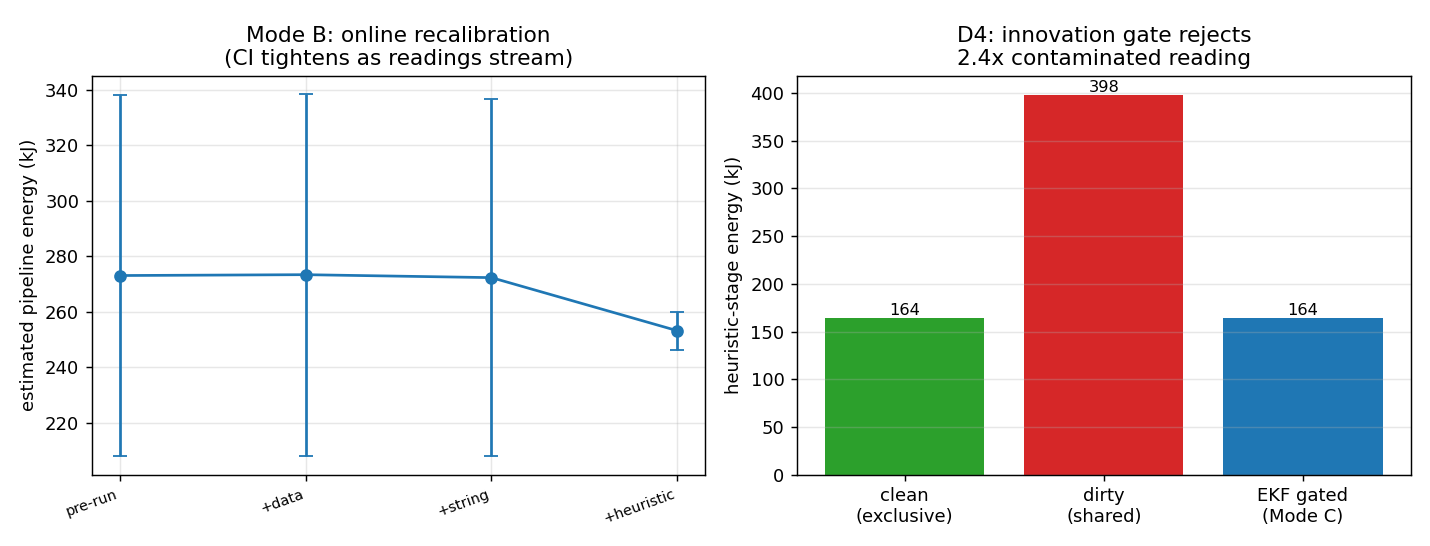
\includegraphics[width=0.92\linewidth]{fig_ekf_estimator.png}
  \caption{The EKF walking the pipeline. Left: the pre-run forecast (Mode~A) and its $95\%$ band tighten as each clean stage reading is absorbed (Mode~B). Right: a contaminated shared-node reading produces a large innovation, trips the $3\sigma$ gate, and is rejected (Mode~C) instead of inflating the total.}
  \label{fig:ekf}
\end{figure}

The final row is the headline. When a contaminated shared-node reading (2.4$\times$ inflated power) is fed to the estimator, the naive sum-of-observations over-estimates the pipeline total by $93\%$. The innovation gate detects the $3\sigma$ discrepancy and falls back to the model prediction, limiting the error to $8\%$. This is the mechanism that converts an unreliable measurement layer into a useful prediction, \emph{without any human gating or manual flagging of bad readings.}

\subsection{Why shared-node power is contaminated --- the controlled experiment}

\label{sec:controlled}

The EKF gate only works if the calibration prior is trustworthy, and the prior is only trustworthy if calibrated on clean data. We tested whether ``clean'' per-job power exists on shared nodes at all. Table~\ref{tab:controlled} shows the result.

\begin{table}[ht]
  \centering
  \begin{tabular}{lrrrr}
    \toprule
    & DC power (W) & Wall time (s) & CPU util. & Energy (kJ) \\
    \midrule
    Exclusive & 275 & 595 & 97\% & 164 \\
    Shared    & \textbf{669} & 595 & 97\% & \textbf{398} \\
    \bottomrule
  \end{tabular}
  \caption{Same stage (\texttt{heuristic\_filtering}), same corpus, same size (100k) --- exclusive vs.\ shared.}
  \label{tab:controlled}
\end{table}

Identical work, identical time, identical utilisation, $2.4\times$ the power. The extra 394\,W is the neighbours on the other cores. \texttt{DC\_NODE\_POWER} is a whole-node BMC reading and does not attribute energy per job on shared nodes. The cgroup-clean counters (\texttt{CPU\_UTIL}, \texttt{CPI}, \texttt{IO\_MBS}) are co-tenancy-immune, but every power signal (\texttt{DC\_NODE\_POWER}, \texttt{PCK\_POWER}, \texttt{MEM\_GBS}) is shared-hardware-level and contaminated. This finding is not a modelling assumption --- it is a measured fact that decides the architecture of the estimator.

\subsection{Shared-node resolution: drive the estimate from time, not power}

\label{sec:results-shared}

We cannot use exclusive nodes in production, and calibrating on contaminated shared power gives $45.8\%$ mean held-out error. First we checked whether \emph{any} clean per-job power signal exists on these nodes: a non-negative least-squares power model on the co-tenancy-immune counters (\texttt{CPU\_UTIL}, \texttt{IO\_MBS}) reaches only $R^2 = 0.08$ --- node idle baselines swing $232$--$640$\,W and bury the $50$--$90$\,W of job-attributable dynamic power. Per-job power is simply not recoverable here. Energy against wall time, by contrast, is clean: $E = P^{\mathrm{eff}} \cdot t$ fits at $R^2 = 0.99$ with a stable per-stage $P^{\mathrm{eff}}$ ($293$, $297$, $278$\,W; ${\approx}290$\,W overall). Since the controlled experiment showed $t_s$ is co-tenancy-invariant, we compute $\hat{E}_s = P^{\mathrm{eff}}_s \cdot t_s$ for every shared run using only the clean wall time. Table~\ref{tab:timedriven} and Figure~\ref{fig:shared} show the result.

\begin{table}[ht]
  \centering
  \begin{tabular}{lrrr}
    \toprule
    Stage & $P^{\mathrm{eff}}$ (W) & Power-based MRE & Time-based MRE \\
    \midrule
    \texttt{data\_splitting}       & $293$ & $54.2\%$ & $12.9\%$ \\
    \texttt{string\_normalization} & $297$ & $20.3\%$ & $\phantom{0}3.0\%$ \\
    \texttt{heuristic\_filtering}  & $278$ & $63.1\%$ & $\phantom{0}0.2\%$ \\
    \midrule
    Overall                        &       & $45.8\%$ & $\mathbf{5.4\%}$ \\
    \bottomrule
  \end{tabular}
  \caption{Shared-node calibrate$\to$predict error: power-based vs.\ time-based. $P^{\mathrm{eff}}$ is calibrated once on the exclusive archive.}
  \label{tab:timedriven}
\end{table}

\begin{figure}[ht]
  \centering
  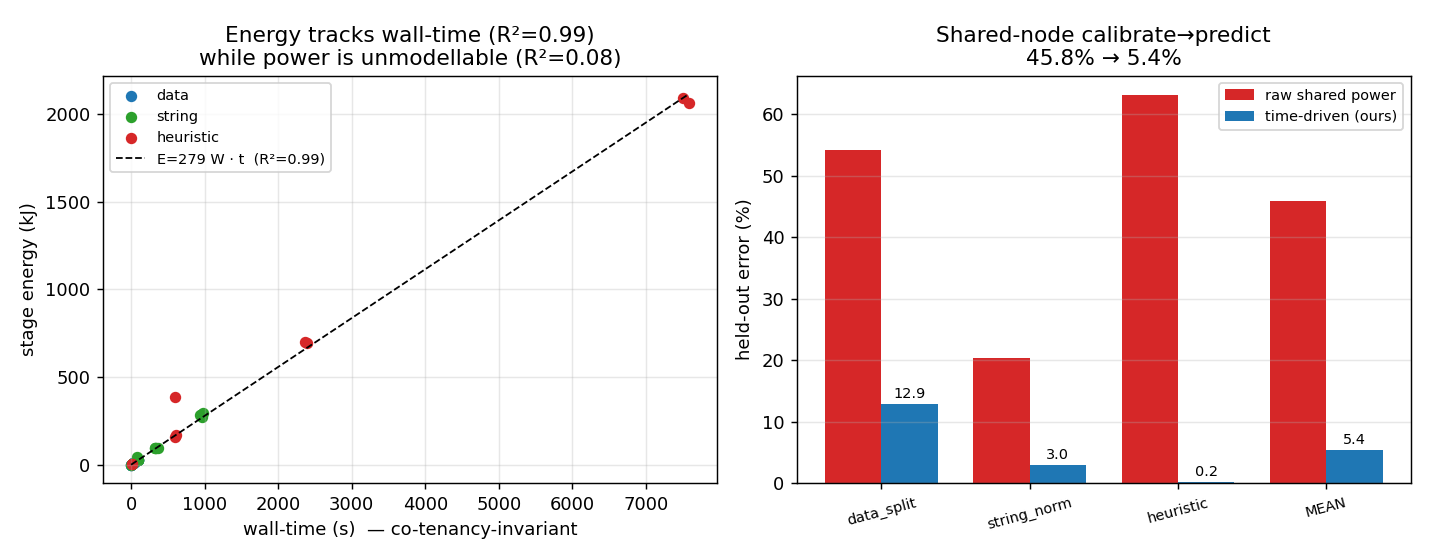
\includegraphics[width=0.92\linewidth]{fig_shared_node.png}
  \caption{Left: stage energy tracks wall time at $R^2 = 0.99$ (a single slope, ${\approx}290$\,W, fits all three stages), while a per-job power model reaches only $R^2 = 0.08$. Right: driving the estimate from time instead of power cuts the shared-node held-out error from $45.8\%$ to $5.4\%$.}
  \label{fig:shared}
\end{figure}

With time-driven estimates, the EKF is re-wired from reject to clean-then-update: Mode~B ingests time-derived energy from every shared run, using $100\%$ of shared data instead of discarding it. On a shared 400k-document run, the re-wired EKF totals $762$\,kJ from cleaned readings vs.\ the $1141$\,kJ ($1.5\times$ inflated) that raw node power would have injected. \textbf{Exclusive is needed zero times going forward.}

\subsection{Cross-corpus transfer: characters, not documents, are the unit of energy}

\label{sec:results-chars}

Within one corpus, $n$ and the total character count $C = n \cdot \bar{\ell}$ are indistinguishable because $\bar{\ell}$ is constant --- their Pearson correlation over our four sizes is $r = 0.9997$. No single-corpus experiment can decide whether a stage scales as $n$ or as $n \log n$, because the two features are near-collinear. A second corpus with a very different document length breaks this.

We ran \emph{European Parliament} ($\bar{\ell} \approx 2.3{\times}10^5$\,characters/document, vs.\ ${\approx}900$ for American Stories --- a $256\times$ difference) through the same pipeline. Table~\ref{tab:chars} shows the result.

\begin{table}[ht]
  \centering
  \begin{tabular}{lcc}
    \toprule
    Stage & am-stories (J/char) & euparl (J/char) \\
    \midrule
    \texttt{string\_normalization} & $4.5{\times}10^{-4}$ & $3.9{\times}10^{-4}$ \\
    \bottomrule
  \end{tabular}
  \caption{Energy per character for the dominant stage across two corpora with a $256\times$ difference in mean document length.}
  \label{tab:chars}
\end{table}

Energy per character agrees to within $12\%$ across the two corpora for the dominant stage (\texttt{string\_normalization}: $4.5{\times}10^{-4}$ vs.\ $3.9{\times}10^{-4}$\,J/char), despite the $256\times$ gap in document length. The feature that generalises across corpora is therefore the total character count $C$, not the document count $n$. You calibrate once on any corpus, read the mean document length of the target corpus, and predict its curation energy by multiplying per-character cost by total characters. The EKF's Mode~B updates then absorb whatever residual corpus-specific offset remains, tightening the estimate as real stages complete. We treat this as a strong observed pattern rather than a confirmed law: euparl is a single size with one replicate (\S\ref{sec:limitations}).

\subsection{Deduplication: the stage that hid, and the stage that does not scale}

\label{sec:results-dedup}

Deduplication runs as four chained sub-jobs --- \texttt{signature} (MinHash signatures), \texttt{buckets} (LSH banding), \texttt{cluster} (connected components), \texttt{filter} (drop duplicates) --- and in the configuration we inherited none of them produced an EAR record: the sub-job launcher never created the directory EAR writes its per-job database into, so the writes silently failed. A single \texttt{mkdir} per sub-job fixes it. With telemetry restored we swept the stage on \emph{exclusive} nodes (clean power) over the same sizes as the other stages. Table~\ref{tab:dedup} reports the per-size energy.

\begin{table}[ht]
  \centering
  \begin{tabular}{lrr}
    \toprule
    Documents & Dedup energy (kJ) & \texttt{signature} share \\
    \midrule
    $10^3$            & $\phantom{00}9.9$ & $35\%$ \\
    $10^5$            & $34.8$            & $73\%$ \\
    $4{\times}10^5$   & $125.6$           & $84\%$ \\
    \bottomrule
  \end{tabular}
  \caption{Deduplication energy, clean exclusive sweep (mean of two replicates; $E = \bar{P}_{\mathrm{dc}}\cdot\Delta t$ at ${\approx}280$\,W). The \texttt{signature} pass dominates and grows from $35\%$ at $10^3$ to $84\%$ at $4{\times}10^5$. The $1.4$M run is absent because it fails out-of-memory (discussed below).}
  \label{tab:dedup}
\end{table}

Three things matter. First, the stage is now a clean measured curve ($c_0=7.9$\,kJ, $c_1=0.29$\,J/doc, Table~\ref{tab:insample}) that feeds the EKF directly. Second, the energy concentrates in \texttt{signature} --- the one sub-job that reads and hashes every surviving document --- so a dedup model only needs to capture that pass; \texttt{buckets} and \texttt{cluster} operate on compact signature tables and are rounding error at scale. Third, the contamination story repeats here: an earlier single dedup run on a co-tenanted node reported $63.5$\,kJ at $100$k, a $1.8\times$ over-read of the clean $34.8$\,kJ --- so dedup energy, like every stage, must be read off clean power (or wall-time), never raw node power.

The $1.4$M run is the one place the pipeline breaks: the signature pass holds all MinHash signatures in memory and is killed out-of-memory after ${\approx}17$ minutes. Running the \emph{whole} pipeline surfaced this --- a three-stage study would not have. It is an engineering limit (the signature builder needs to spill to disk or shard), and it bounds where the linear dedup model is usable: $1$k--$400$k today, pending a memory fix.

% ===========================================================================
\section{Limitations and Future Work}
% ===========================================================================

\label{sec:limitations}

\textbf{Replicate depth.} The calibration sweep has two replicates per (stage, size) cell, so noise estimates are coarse. Three to five replicates would tighten the per-stage prediction intervals by ${\sim}30\%$.

\textbf{Deduplication scaling and the memory wall.} Deduplication is now swept cleanly at $1$k--$400$k (\S\ref{sec:results-dedup}), where it is well described by the linear model (held-out $R^2=0.96$). But the $1.4$M run fails out-of-memory in the signature pass, so we cannot yet quote the model past $4{\times}10^5$ documents. Fixing this (spill-to-disk or sharding the MinHash signature builder) and then extending the sweep to $1.4$M --- where any $O(n\log n)$ curvature would show --- is the priority follow-up, since deduplication is on the critical path of every production run.

\textbf{Cross-corpus scope.} The European Parliament result is preliminary (few sizes, single replicate). A denser multi-corpus sweep with ${\ge}3$ corpora and ${\ge}3$ replicates per size would convert the character-invariance finding from an observed pattern into a confirmed law.

\textbf{GPU stages.} All stages here are CPU-only. The GPT-NL pipeline includes two GPU stages (PII masking, toxic language detection) running on A100 and H100 partitions; their energy models require separate calibration on those partitions.

\textbf{Node idle variability.} Light single-core stages on exclusive nodes are dominated by the idle draw of the remaining 191 reserved cores ($232$--$640$\,W across nodes). Per-core attribution via shared-node CPU-share energy (reading \texttt{eacct} on genuinely shared jobs, not exclusive ones) is the measurement-side fix.

% ===========================================================================
\section{Conclusion}
% ===========================================================================

We built a whole-pipeline energy account for the four-stage GPT-NL data-curation pipeline. Each stage is calibrated cheaply on exclusive nodes; an EKF then walks the pipeline and its innovation gate automatically rejects contaminated or missing EAR readings. Across all four stages, held-out prediction $R^2 = 0.73$--$0.96$; the gate cuts a contaminated reading's $+93\%$ pipeline error to $+8\%$; a cross-corpus per-character energy invariant (${\approx}4{\times}10^{-4}$\,J/char) makes the prior portable; and deduplication --- once its telemetry was fixed --- is measured cleanly at $1$k--$400$k ($34.8$\,kJ at $100$k, $84\%$ in the signature pass), while its $1.4$M run reveals the one stage that does not scale (out-of-memory in the signature pass). When shared-node power contamination is resolved via the time-driven estimate $E = P^{\mathrm{eff}} \cdot t$, prediction error drops from $45.8\%$ to $5.4\%$ --- so exclusive calibration is needed zero times going forward.

The reason to run the \emph{whole} pipeline, not a convenient subset, is that the total is what the team must budget --- and it is exactly the awkward-to-measure stage (deduplication) that both hid from the telemetry and broke at scale. Model what you can calibrate cheaply, walk what you must predict, gate what you cannot trust, and the full-pipeline number stays honest even when the measurement infrastructure is partially broken.

% ===========================================================================
% Bibliography
% ===========================================================================

\bibliographystyle{plainnat}
\bibliography{references}

\end{document}
